\documentclass[ignorenonframetext]{beamer}
\usetheme{metropolis}
\usepackage{amssymb,amsmath}
\definecolor{links}{HTML}{CCCC00}
\hypersetup{colorlinks,linkcolor=,urlcolor=links}
\usepackage[T1]{fontenc}
\usepackage[utf8]{inputenc}
\usepackage{microtype}
\usepackage{longtable, booktabs}
\usepackage[english]{babel}
\usepackage{pgf, microtype, booktabs, times, etex}
\usepackage{tcolorbox}
\tcbuselibrary{minted,skins}

\newtcblisting{latexcode}{
	listing engine=minted,
	colback=bashcodebg,
	colframe=black!70,
	listing only,
	minted style=colorful,
	minted language=latex,
	minted options={linenos=true,texcl=true},
	left=1mm,
}
\definecolor{bashcodebg}{rgb}{0.85,0.85,0.85}
%\usemintedstyle{emacs}
\beamertemplatenavigationsymbolsempty

\title{Open source \& data sharing}
\subtitle{Or \ldots how to stop worrying and leverage your research}
\author{Thomas de Graaff}
\institute{Department of Spatial Economics}
\date{June 23, 2020}

\begin{document}

\frame{\titlepage}

\begin{frame}
  \frametitle{Open source---free as in beer, not in time!}
    \centering
    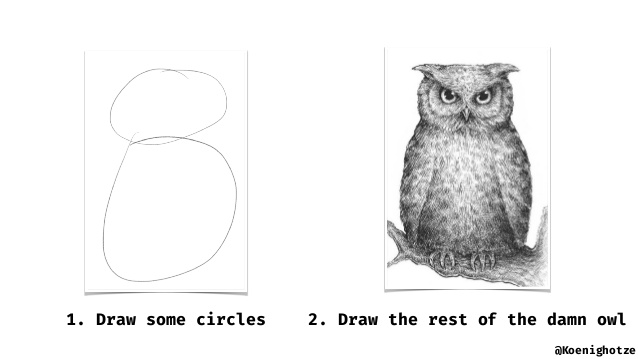
\includegraphics[width = 1\textwidth]{owl.jpg}
  \end{frame}

\begin{frame}
  \frametitle{What I advocate}
  \begin{columns}
    \begin{column}{.5\textwidth}
      To make available online and for anyone to \alert{access}, \alert{assess}, \alert{reuse} \& \alert{contribute} to:
      \begin{itemize}
        \item All your \alert{data}. And, if not possible
          \begin{itemize}
            \item metadata
            \item subset
            \item simulated/scrambled data
          \end{itemize}
        \item All \alert{text} files, including scripts, figures, working paper\pause
        \end{itemize}
    \end{column}

    \begin{column}{.5\textwidth}
      So, why `give' it away?
      \begin{itemize}
        \item The greater good: \alert{transparency} \& \alert{reproducibility}
          \begin{itemize}
            \item avoid ``additional results available upon request''
          \end{itemize}
        \item \alert{Private} gains:
          \begin{itemize}
            \item higher visibility (others will actually use your research)
              \begin{itemize}
                \item Nunn \& Puga (Restat, 2012)
              \end{itemize}
              \item incentives on working `tidy'
          \end{itemize}
      \end{itemize}
    \end{column}
  \end{columns}
\end{frame}

\begin{frame}
  \frametitle{How can I do that?}
    \begin{columns}
    \begin{column}{.5\textwidth}
      \begin{itemize}
        \item Using a \alert{versioning} system and an online platform
          \begin{itemize}
\item To \alert{share}, \alert{distribute} and \alert{cooperate} on data\newline
          \end{itemize}
          \item Currently, \alert{Git} and \alert{GitHub} is the default (but Bitbucket, etc.)\newline
          \item Complete version history with time stamps\pause
      \end{itemize}
    \end{column}

    \begin{column}{.5\textwidth}
       \begin{itemize}
        \item You work on a piece (data) and using Git \alert{commit} to your own local repository
        \item Then you push to an \alert{open} online repository (GitHub)
        \item Which now serves as your (ugly) website as well
          \begin{itemize}
            \item Actually people (well, me) blog using GitHub as a free server using Jekyll or Hugo (blogdown)
          \end{itemize}
      \end{itemize}
    \end{column}
  \end{columns}
\end{frame}

\begin{frame}
  \frametitle{Applications for Git/GitHub}

  \begin{columns}
      \begin{column}{.5\textwidth}
      \begin{itemize}
        \item GUI applications
          \begin{itemize}
            \item GitHub desktop, GitKraken, ScourgeTree \newline
          \end{itemize}
        \item Built-in most proper editors:
          \begin{itemize}
            \item Sublime, Emacs, Overleaf, RStudio, etc.\newline
          \end{itemize}
          \item Command line (most powerful, but \ldots)
        \end{itemize}
    \end{column}

    \begin{column}{.5\textwidth}
      \begin{figure}[h]
        \centering
        
\includegraphics[width = 1\textwidth]{octopussy}
        \end{figure}
    \end{column}
  \end{columns}

\end{frame}

\begin{frame}
  \frametitle{Package it!}
  Instead of just providing the data you can wrap it in an \alert{(R-)package}
  \begin{itemize}
    \item give examples (vignettes) of the code and data
    \item data easier to read
    \item distribution via CRAN or \alert{GitHub}\newline
  \end{itemize}
  Many R-packages contain (access) to economic data
  \begin{itemize}
    \item \texttt{AER} package---all applied econometrics textbook data (California test score data...)
    \item \texttt{IMFData}
    \item \texttt{wbstats}---World bank data
  \end{itemize}

\end{frame}

\begin{frame}[standout]
  Presentation can be found on:

  \url{https://github.com/Thdegraaff/Datasharing_presentation}
\end{frame}

\end{document}

%%% Local Variables:
%%% LaTeX-command: "latex -shell-escape"
%%% End:
